\section{Resultados}
Terminaron las 144 ejecuciones previstas. La auditoría reconcilia 416 llamadas y 568\,283 tokens informados por el proveedor, incluidas las 24 ejecuciones de carga de skills. Hubo 0 errores de infraestructura o ejecución del protocolo; todas las ejecuciones tienen consumo completo. Se excluyen las seis del piloto. Los hashes iniciales y finales coinciden y el orden registrado corresponde al plan fijado.

Se evaluó el 13 de septiembre de 2026 entre 13:09:45 y 13:33:34 UTC. Son tiempos observados ese día contra la API, no una previsión para otras cuentas o despliegues.

\begin{table}[htbp]
\centering\small
\setlength{\tabcolsep}{4pt}
\begin{tabular}{@{}lrrrrr@{}}
\toprule
\textbf{Configuración} & \textbf{Estricto} & \textbf{SQL norm.} & \textbf{Tokens/ej.} & \textbf{Media s} & \textbf{Mediana s}\\
\midrule
Agente único & 20/24 & 23/24 & 1\,143 & 4.72 & 3.39\\
Secuencial & 20/24 & 24/24 & 3\,410 & 13.72 & 11.77\\
Paralela & 19/24 & 23/24 & 3\,520 & 8.14 & 6.04\\
Jerárquica & 20/24 & 24/24 & 4\,373 & 11.19 & 10.01\\
Reflexiva & 20/24 & 24/24 & 2\,714 & 9.77 & 6.26\\
\midrule
Jerárquica + todos los skills & 21/24 & 24/24 & 8\,518 & 11.93 & 10.88\\
\bottomrule
\end{tabular}
\caption{Resultados observados. Estricto es el criterio principal fijado. SQL norm. es la sensibilidad posterior al envoltorio; no cambia el texto de la consulta. La última fila separada corresponde a la carga de skills.}
\label{tab:results}
\end{table}

\subsection{Cumplimiento de formato y calidad de la solución}
Durante la evaluación, las respuestas SQL mostraron una diferencia entre una consulta aparentemente correcta y la estructura anidada solicitada. Se conservó el evaluador principal. Una sensibilidad explícitamente posterior envuelve una cadena existente dentro de answer en un objeto con campo sql y ejecuta la misma consulta contra las tres bases. No se corrige ni repite texto SQL, respuesta numérica, prompt o intento.

La normalización se aplica a 22 salidas registradas y cambia los aciertos completos de 120/144 a 142/144 entre las seis configuraciones. La columna estricta mide también cumplimiento del formato entregado; la normalizada diagnostica cuánto fallo se atribuye al envoltorio. No es otro objetivo prefijado ni prueba de que todas las consultas funcionen fuera de estas bases.

Los dos fallos restantes corresponden a T05, repetición 2, en las configuraciones individual y paralela. Ambas entregan la duración total correcta de 38, pero inician H en 10 en vez de 18 y K en 21 en vez de 29. H depende de que termine C y K de que termine H. Es un error al propagar dependencias, no de envoltorio JSON; comprobar solo la duración final lo ocultaría.

\begin{figure}[htbp]
\centering
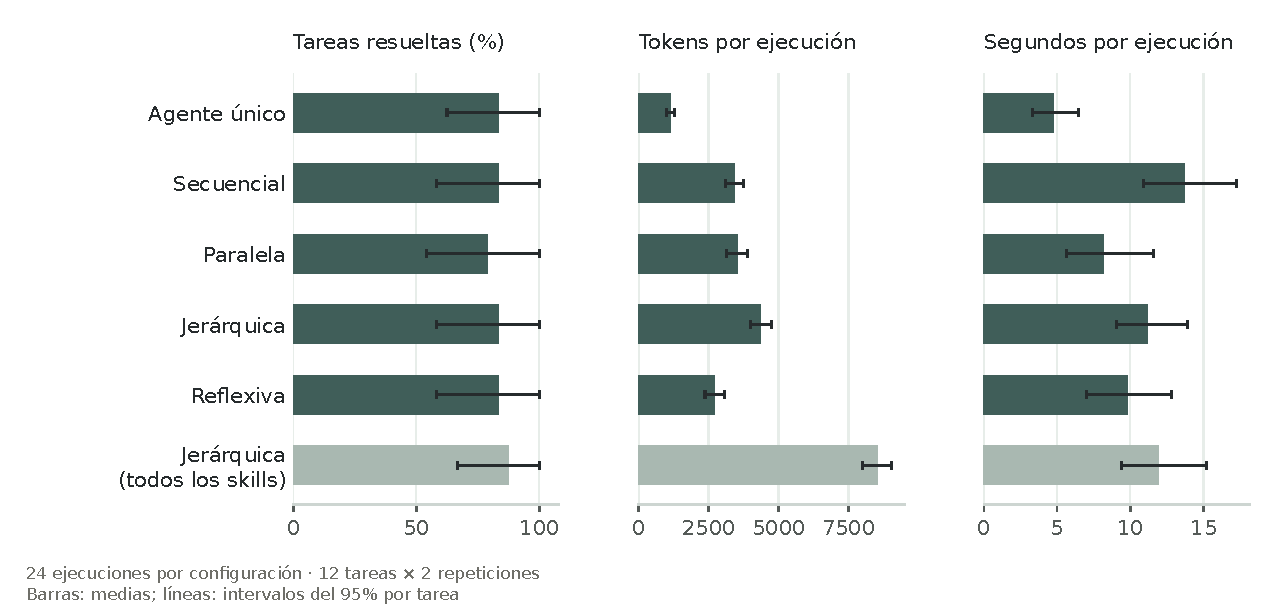
\includegraphics[width=\linewidth]{../../results/analysis/comparison-es.pdf}
\caption{Éxito principal, tokens totales y tiempo transcurrido medidos. Las líneas muestran intervalos descriptivos del 95\% por tarea. La carga de todos los skills se distingue del resto. Figura generada con los datos entregados.}
\label{fig:comparison}
\end{figure}

\subsection{Skills seleccionados frente al catálogo completo}
La configuración jerárquica consume 4\,373 tokens medios con un skill seleccionado y 8\,518 al cargar los diez cuerpos. La diferencia media pareada es 4\,145 tokens, con intervalo del 95\% [3898; 4366]. El incremento es 94.8\%, intervalo [87.9; 101.9]\%.

El éxito estricto pasa de 20/24 a 21/24; con la sensibilidad de envoltorio pasa de 24/24 a 24/24. La diferencia media de latencia, todos menos seleccionado, es 0.74 segundos, intervalo [-0.24; 1.83]. Es una comparación de carga con el grupo correcto conocido de antemano; no mide errores de búsqueda de skills ni su coste.

\subsection{Costes e incertidumbre}
El flujo reflexivo ejecuta 5 llamadas de revisión en 24 ejecuciones; un crítico puede añadir coste aunque no haya revisión posterior. La API informa 44\,788 tokens de entrada cacheada y 97\,915 de razonamiento. Son subconjuntos, no tokens adicionales. Las tablas~\ref{tab:efficiency} y~\ref{tab:intervals} conservan intentos fallidos y reflejan el pequeño número de instancias independientes. Un orden puntual no establece superioridad general estadística.

\begin{table}[htbp]
\centering\small
\setlength{\tabcolsep}{4pt}
\begin{tabular}{@{}lrrrr@{}}
\toprule
\textbf{Configuración} & \textbf{Tokens totales} & \textbf{Llamadas} & \textbf{Aciertos/100k tok.} & \textbf{Aciertos/min}\\
\midrule
Agente único & 27\,424 & 24 & 72.93 & 10.58\\
Secuencial & 81\,845 & 72 & 24.44 & 3.64\\
Paralela & 84\,479 & 72 & 22.49 & 5.83\\
Jerárquica & 104\,963 & 95 & 19.05 & 4.47\\
Reflexiva & 65\,133 & 58 & 30.71 & 5.12\\
\midrule
Jerárquica + todos los skills & 204\,439 & 95 & 10.27 & 4.40\\
\bottomrule
\end{tabular}
\caption{Eficiencia con aciertos estrictos y todos los intentos. Aciertos por minuto acumulado no equivale a capacidad de un servidor saturado.}
\label{tab:efficiency}
\end{table}

\begin{figure}[htbp]
\centering
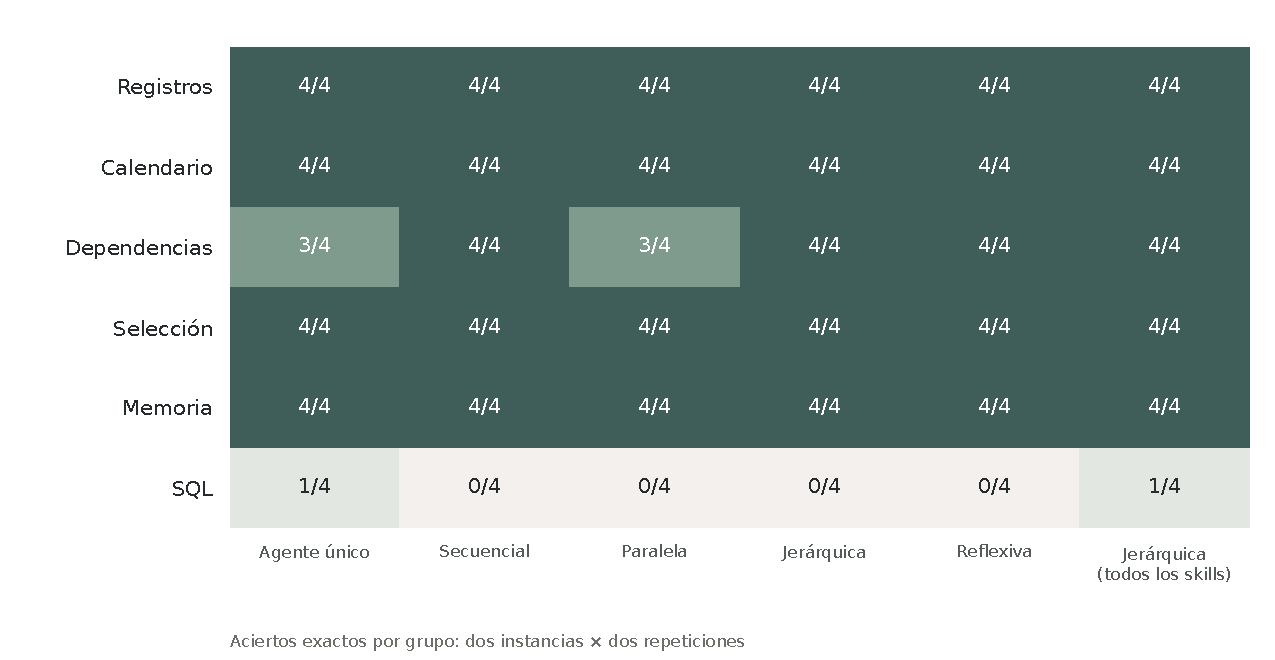
\includegraphics[width=\linewidth]{../../results/analysis/families-es.pdf}
\caption{Aciertos estrictos por grupo. Cada celda corresponde a cuatro ejecuciones, no cuatro instancias independientes. La sensibilidad SQL figura por separado en la tabla~\ref{tab:results}.}
\label{fig:families}
\end{figure}

\begin{table}[htbp]
\centering\small
\setlength{\tabcolsep}{4pt}
\begin{tabular}{@{}lrrr@{}}
\toprule
\textbf{Configuración} & \textbf{Éxito \%} & \textbf{Tokens medios} & \textbf{Segundos medios}\\
\midrule
Agente único & [62.5; 100.0] & [1005; 1279] & [3.33; 6.43]\\
Secuencial & [58.3; 100.0] & [3094; 3752] & [10.90; 17.28]\\
Paralela & [54.2; 100.0] & [3157; 3904] & [5.65; 11.58]\\
Jerárquica & [58.3; 100.0] & [4012; 4740] & [9.04; 13.89]\\
Reflexiva & [58.3; 100.0] & [2373; 3064] & [7.03; 12.82]\\
Jerárquica + todos los skills & [66.7; 100.0] & [7987; 9037] & [9.39; 15.22]\\
\bottomrule
\end{tabular}
\caption{Intervalos descriptivos del 95\% por bootstrap de tareas para éxito principal, tokens medios y tiempo medio. Se remuestrean doce identificadores de tarea.}
\label{tab:intervals}
\end{table}
